\documentclass[11pt]{beamer}
\usetheme{CambridgeUS}
%\usepackage[utf8]{inputenc}
%\usepackage[turkish]{babel}
\usepackage{amsmath}
\usepackage{amsfonts}
\usepackage{amssymb}
\usepackage{graphicx}
\usepackage{listings}
\usepackage{tikzsymbols}
\usepackage{tikz-network}
\usepackage{tikzlings}


\definecolor{lbcolor}{rgb}{0.99,0.99,0.95}  
\lstset{  
	language=Python,  
	tabsize=4,  
	basicstyle=\ttfamily,  
	backgroundcolor=\color{lbcolor},  
	showstringspaces=false,
	frame=single,
	frameround=tttt
}


\author{Prof.Dr.Mehmet Hakan Satman \\ mhsatman@istanbul.edu.tr}
\title{Scientific Computing and (Big) Data Analysis with Julia}
\setbeamercovered{transparent} 
%\setbeamertemplate{navigation symbols}{} 
\logo{
\includegraphics[width=1cm]{images/iulogo.jpg}} 
\institute{Istanbul University} 
\date{2023.12.01} 

\begin{document}

\begin{frame}

\includegraphics[width=1cm]{images/julia.png}
\titlepage
\end{frame}


\begin{frame}[fragile]{Julia Programming Language}{julialang.org}
	\begin{center}
		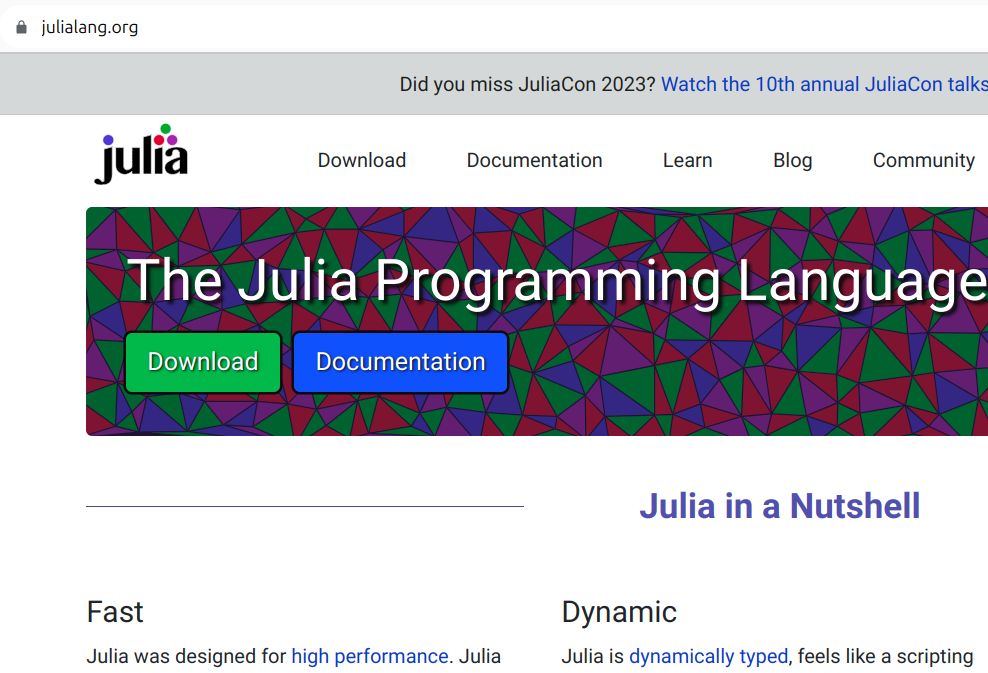
\includegraphics[width=8cm]{images/thesite.png}
	\end{center}
\end{frame}

\section{What is Julia}
\begin{frame}[fragile]{Julia Programming Language}{High Performance Computing \& Dynamic}
\begin{itemize}
	\item Julia was designed for high performance. Julia programs automatically compile to efficient native code via LLVM, and support multiple platforms (Windows, MacOS, Linux, etc.).
	
	\item Julia is dynamically typed, feels like a scripting language, and has good support for interactive use, but can also optionally be separately compiled\footnote{\url{https://julialang.org/}}.
\end{itemize}
\end{frame}



\begin{frame}[fragile]{Julia Programming Language}{Composable \& Open Source}
	\begin{itemize}
		\item Julia uses multiple dispatch as a paradigm, making it easy to express many object-oriented and functional programming patterns. The talk on the Unreasonable Effectiveness of Multiple Dispatch explains why it works so well.
		\item Julia is an open source project with over 1,000 contributors. It is made available under the MIT license. The source code is available on GitHub\footnote{\url{https://julialang.org/}}.
	\end{itemize}
\end{frame}


\begin{frame}[fragile]{Julia Programming Language}{Compilation to Binary}
Julia code is compiled into binary executable via LLVM (Low-Level Virtual Machine).
	\begin{center}
			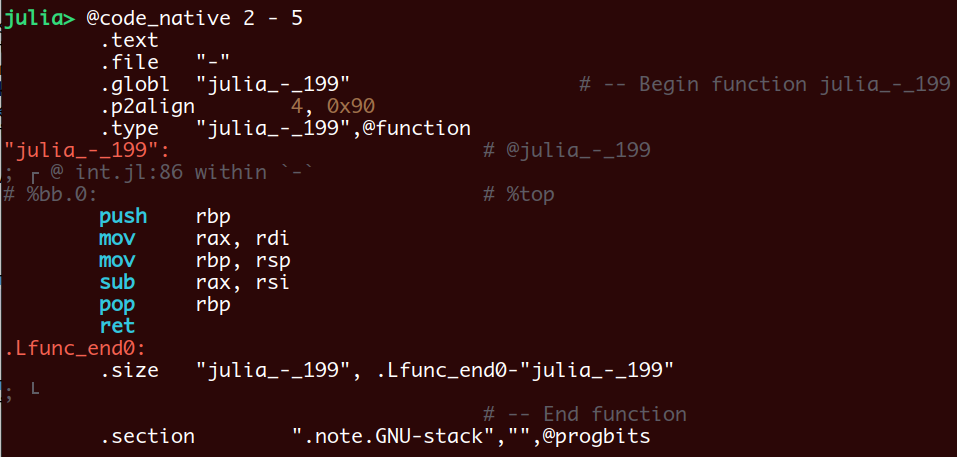
\includegraphics[width=10cm]{images/assembly.png}
	\end{center}
\end{frame}


\begin{frame}[fragile]{Julia Programming Language}{First things first!}
\begin{exampleblock}{helloworld.jl file}
\begin{lstlisting}
	println("Hello, world!")
\end{lstlisting}
\end{exampleblock}

\begin{lstlisting}
julia> include("helloworld.jl")
Hello, world!
\end{lstlisting}

\end{frame}

\subsection{The setup}
\begin{frame}[fragile]{Julia Programming Language}{Welcome!}
	\begin{center}
			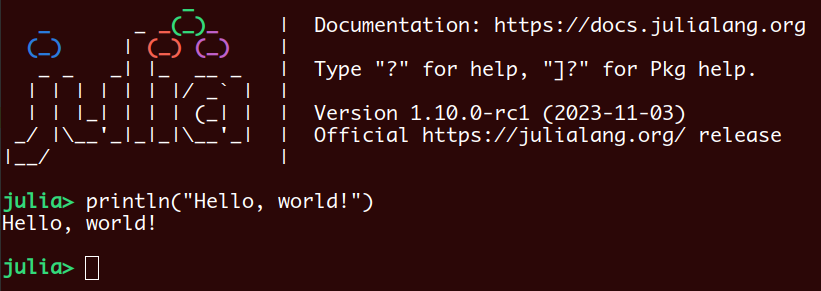
\includegraphics[width=10cm]{images/welcome.png}
	\end{center}
\end{frame}


\begin{frame}[fragile]{Julia Programming Language}{The editor: Visual Studio Code}
	\begin{center}
		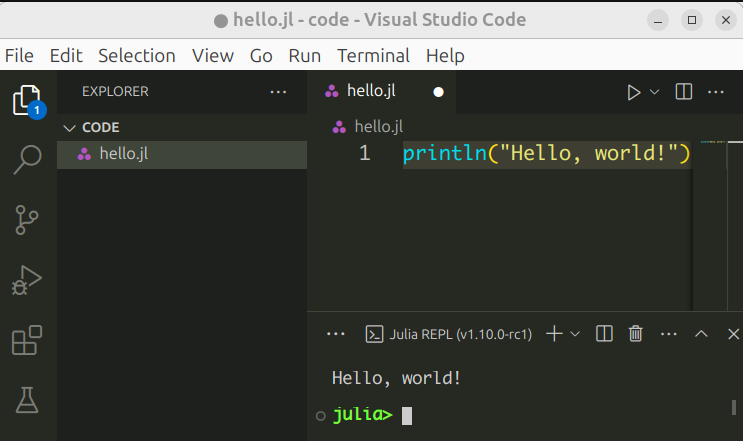
\includegraphics[width=10cm]{images/vscode.png}
	\end{center}
\end{frame}

\section{Language basics}
\begin{frame}[fragile]{Julia Programming Language}{Basics}
Variables have types (Int, Float, Bool, String, etc.)
\begin{lstlisting}
julia> a = 3
3
julia> b = 3.14159265
3.14159265
julia> typeof(a)
Int64
julia> typeof(b)
Float64
\end{lstlisting}
\end{frame}

\subsection{Vectors and Matrices}
\begin{frame}[fragile]{Julia Programming Language}{Vectors}
Vectors and Matrices are first-class citizens (no need for external libs)
\begin{lstlisting}
julia> v = [1, 42, -8, 10]
4-element Vector{Int64}:
1
42
-8
10
\end{lstlisting}
\end{frame}


\begin{frame}[fragile]{Julia Programming Language}{Matrices}
\begin{lstlisting}
julia> hcat(zeros(5), ones(5), 1:5, 5:(-1):1)
5x4 Matrix{Float64}:
 0.0  1.0  1.0  5.0
 0.0  1.0  2.0  4.0
 0.0  1.0  3.0  3.0
 0.0  1.0  4.0  2.0
 0.0  1.0  5.0  1.0
\end{lstlisting}
\end{frame}

\begin{frame}[fragile]{Julia Programming Language}{Matrices}
\begin{lstlisting}
julia> m = zeros(5, 3)
5x3 Matrix{Float64}:
0.0  0.0  0.0
0.0  0.0  0.0
0.0  0.0  0.0
0.0  0.0  0.0
0.0  0.0  0.0

julia> size(m)
(5, 3)
\end{lstlisting}
\end{frame}

\subsection{Importing Data}

\begin{frame}[fragile]{Julia Programming Language}{Installing packages}
\begin{lstlisting}
julia> using Pkg
julia> Pkg.add("JMcDM")
\end{lstlisting}

\begin{lstlisting}
julia> ]
@v1.10) pkg> add JMcDM
\end{lstlisting}
\end{frame}

\begin{frame}[fragile]{Julia Programming Language}{Importing Data}
\begin{lstlisting}
using CSV, DataFrames

mydata = CSV.read("data.csv", 
				   delim = ";", 
				   DataFrame)

show(mydata)
\end{lstlisting}
\end{frame}


\begin{frame}[fragile]{Julia Programming Language}{Importing Data}
\begin{lstlisting}
julia> using Latexify
julia> latexify(mydata, env = :table) |> println
\end{lstlisting}

\begin{tabular}{cc}
$X$ & $ Y$\\
$1$ & $2$\\
$2$ & $4$\\
$3$ & $5$\\
$4$ & $-1$\\
$5$ & $2$\\
\end{tabular}

\end{frame}


\subsection{Flow Control}
\begin{frame}[fragile]{Julia Programming Language}{if/elseif/else}
\begin{lstlisting}
function numberofrealroots(delta)
	if delta > 0 
		return 2
	elseif delta == 0
		return 1
	else
		return 0
	end
end  
\end{lstlisting}
\end{frame}

\begin{frame}[fragile]{Julia Programming Language}{Pattern Matching}
\begin{lstlisting}
using Rematch

function numberofrealroots(delta)
    @match delta begin
        x where x > 0  => 2
        x where x == 0 => 1
        _              => 0
    end 
end
\end{lstlisting}
\end{frame}


\begin{frame}[fragile]{Julia Programming Language}{Sum Types a.k.a. tagged unions (just like enum in Rust)}
\begin{lstlisting}[basicstyle=\tiny]
using  SumTypes 

@sum_type Expression begin
    ConstantI64(::Int64)
    Add(::Expression, ::Expression)
end

function eval(e::Expression) 
    result = @cases e begin 
        ConstantI64(i) => i 
        Add(e1, e2)    => eval(e1) + eval(e2)
        _              => error("Cannot understand :")
    end 
    return result
end 

eval(Add(ConstantI64(6), ConstantI64(5)))
\end{lstlisting}
\end{frame}


\subsection{For Loops}
\begin{frame}[fragile]{Julia Programming Language}{Loops}
For loops are single threaded by design
\begin{lstlisting}
results = zeros(10)

for i in 1:10
	results[i] = dosomethingwith(i)
end 
\end{lstlisting}
\end{frame}


\subsection{Multi-threaded programming}
\begin{frame}[fragile]{Julia Programming Language}{Threads}
Using multiple threads\footnote{\#\> julia -t 10} 
\begin{lstlisting}
using Base.Threads

results = zeros(10)
	
@threads for i in 1:10
	results[i] = dosomethingwith(i)
end 
\end{lstlisting}
\end{frame}


\subsection{Multi-threaded programming}
\begin{frame}[fragile]{Julia Programming Language}{Distributed Programming}
\begin{lstlisting}
julia> using Distributed
julia> addprocs(5);
julia> pmap(abs, [1, 2, -5, 10, 100, -6])
6-element Vector{Int64}:
   1
   2
   5
  10
 100
   6

\end{lstlisting}
\end{frame}


\subsection{Functions}
\begin{frame}[fragile]{Julia Programming Language}{Functions are first-class citizens}
\begin{lstlisting}
function apply(f, x)
	return f(x)
end 

julia> apply(abs, -10)
10
\end{lstlisting}
\begin{itemize}
\item Functions can take functions as arguments.
\item Functions can return functions as values.
\end{itemize}
\end{frame}


\subsection{Multiple Dispatch}
\begin{frame}[fragile]{Julia Programming Language}{Multiple Dispatch}
\begin{lstlisting}
struct Point2D 
	x::Float64
	y::Float64
end 
\end{lstlisting}
\begin{itemize}
\item Structs are user-defined concrete data types.
\item An object instance can be created like \texttt{Point2D(1, 2)}.
\item Object fields can be accessed like \texttt{p.x} and \texttt{p.y}.
\end{itemize}
\end{frame}


\begin{frame}[fragile]{Julia Programming Language}{Multiple Dispatch}
\begin{lstlisting}[basicstyle=\small]
function Base.:+(p::Point2D, other::Point2D)::Point2D
	Point2D(p.x + other.x, p.y + other.y)
end 
\end{lstlisting}
\begin{lstlisting}
julia> Point2D(1, 2) + Point2D(4, 5)
Point2D(5.0, 7.0)
\end{lstlisting}
\begin{itemize}
\item Operator \texttt{+} is overloaded for the type \texttt{Point2D}.
\item Now, both \texttt{2 + 2} and \texttt{p1 + p2} are legal Julia codes where \texttt{p1} and \texttt{p2} are in type of \texttt{Point2D}.
\end{itemize}
\end{frame}



\begin{frame}[fragile]{Julia Programming Language}{Multiple Dispatch}
\begin{lstlisting}[basicstyle=\small]
function Base.:*(p::Point2D, other::Point2D)::Float64
	return p.x * other.x + p.y * other.x
end 
\end{lstlisting}
\begin{lstlisting}
julia> Point2D(1, 2) * Point2D(4, 5)
12.0
\end{lstlisting}
\begin{itemize}
\item The operator \texttt{*} is overloaded for the type \texttt{Point2D}.
\item \texttt{*} now operates like the \emph{dot product} of vectors in linear algebra.
\end{itemize}
\end{frame}

\begin{frame}[fragile]{Linear Regression}{The formulation}
\begin{equation}
y = \beta_0 + \beta_1 x + \varepsilon
\end{equation}

\begin{equation}
	\hat{y} = \hat{\beta}_0 + \hat{\beta}_1 x 
\end{equation}

\begin{equation}
	\hat{\boldsymbol{\beta}} = (X'X)^{-1}X'y
\end{equation}
\end{frame}


\section{Linear Regression}
\begin{frame}[fragile]{Linear Regression}{Sample Data}
\begin{equation}
X = \begin{bmatrix}
	1 & 1 \\
	1 & 2 \\
	1 & 3 \\
	1 & 4 \\
	1 & 5 
\end{bmatrix}, y = \begin{bmatrix}
2 \\
5 \\ 
5 \\ 
8 \\ 
12
\end{bmatrix}
\end{equation}
\end{frame}


\begin{frame}[fragile]{Linear Regression}{The Matrix Solution}
\begin{lstlisting}
using LinearAlgebra
		
x = [1, 2, 3, 4, 5]
y = [2, 5, 5, 8, 12]
X = hcat(ones(5), x)
betahats = inv(X'X)X'y
println(betahats)
\end{lstlisting}
	
\begin{lstlisting}
julia> include("reg-matrix.jl")
[-0.5, 2.3]
\end{lstlisting}
\end{frame}


\begin{frame}[fragile]{Linear Regression}{Pseudo Inverse - Numerical Fit}
\begin{lstlisting}
x = [1, 2, 3, 4, 5]
y = [2, 5, 5, 8, 12]

betahats = hcat(ones(5), x) \ y 
println(betahats)	
\end{lstlisting}

\begin{lstlisting}
julia> include("reg-simple.jl")
[-0.5, 2.3]
\end{lstlisting}
\end{frame}


\begin{frame}[fragile]{Linear Regression}{The GLM package}
\begin{lstlisting}
using GLM 

x = [1, 2, 3, 4, 5]
y = [2, 5, 5, 8, 12]

result = lm(hcat(ones(5), x), y)

println(result)

\end{lstlisting}
\end{frame}


\begin{frame}[fragile]{Linear Regression}{The GLM package - Results}
\begin{lstlisting}[basicstyle=\tiny]
julia> include("reg-glm.jl")
	
Coefficients:
------------------------------
	  Coef.  Std. Error   t     Pr(>|t|)  Lower 95%  Upper 95%
------------------------------
x1   -0.5    1.25565   -0.40    0.7171   -4.49605    3.49605
x2    2.3    0.378594   6.08    0.0090    1.09515    3.50485
------------------------------
\end{lstlisting}

\begin{lstlisting}
julia> GLM.r2(result)
0.9248251748251748
\end{lstlisting}


\end{frame}


\section{MLJ}
\begin{frame}[fragile]{MLJ}{A Machine Learning Framework for Julia}
\begin{lstlisting}[basicstyle=\tiny]
julia> using MLJ
julia> models = MLJ.models()
julia> for m in models
           println(m[:name])
       end
ARDRegressor
AdaBoostClassifier
AdaBoostRegressor
AdaBoostStumpClassifier
...
KMedoids
KNNClassifier
...
NeuralNetworkRegressor
...
RandomForestClassifier
RandomForestImputer
RandomForestRegressor
...
SRRegressor
\end{lstlisting}
\end{frame}

\subsection{Symbolic Regression}
\begin{frame}[fragile]{XOR}{eXclusive OR}
\begin{table}
\centering
\begin{tabular}{|c|c|c|}
	\hline
	$x_1$ & $x_2$ & $y$ \\
	\hline 
	1 & 1 & 0 \\
	\hline 
	1 & 0 & 1 \\
	\hline 
	0 & 1 & 1 \\
	\hline 
	0 & 0 & 0 \\
	\hline 
\end{tabular}
\caption{$y = \text{xor}(x_1, x_2)$}
\end{table}
\end{frame}

\begin{frame}[fragile]{Symbolic Regression}
\begin{lstlisting}
using SymbolicRegression, MLJ

x = (
	x1 = Float64[1, 1, 0, 0], 
	x2 = Float64[1, 0, 1, 0]
)
		
y = Float64[0, 1, 1, 0]
		
\end{lstlisting}
\end{frame}


\begin{frame}[fragile]{Symbolic Regression}
	\begin{lstlisting}
model = SRRegressor(
	niterations = 50,
	binary_operators = [+, -, *],
	unary_operators = [abs],
	should_simplify = true,
	save_to_file = false)

\end{lstlisting}
\end{frame}

\begin{frame}[fragile]{Symbolic Regression}
\begin{lstlisting}
mach = machine(model, x, y)
fit!(mach)
report(mach)
@info predict(mach, x)
\end{lstlisting}
\end{frame}


\begin{frame}[fragile]{Symbolic Regression}
\begin{lstlisting}
Hall of Fame:   
------------------                                                                                                                                    Complexity  Loss       Score     Equation                                                                                                                1           2.500e-01  3.604e+01  y = 0.5                                                                                                                4           0.000e+00  1.201e+01  y = abs(x1 - x2)
--------------------                                                                                                       
[ Info: [0.0, 1.0, 1.0, 0.0]

\end{lstlisting}
\end{frame}

\section{A Short Break}
\begin{frame}[fragile]{}
\begin{center}
\Coffeecup[7] \\
\vspace{1cm}
{\huge
\begin{quotation}
one more cup of coffee?
\end{quotation}
} 
\end{center}
\end{frame}

\section{Clustering Multivariate Data}
\begin{frame}[fragile]{Clustering Multivariate Data}{kmedoids}
	\begin{center}
		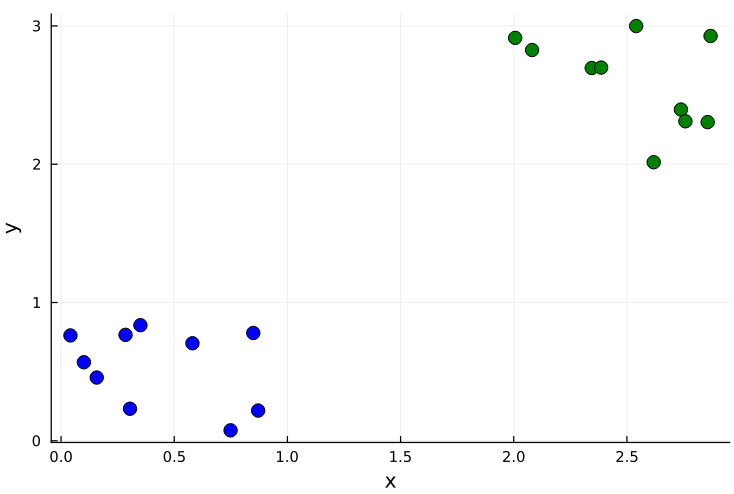
\includegraphics[width=8cm]{images/kmedoids1.png}
	\end{center}
\end{frame}

\begin{frame}[fragile]{Clustering Multivariate Data}{kmedoids}
	\begin{center}
		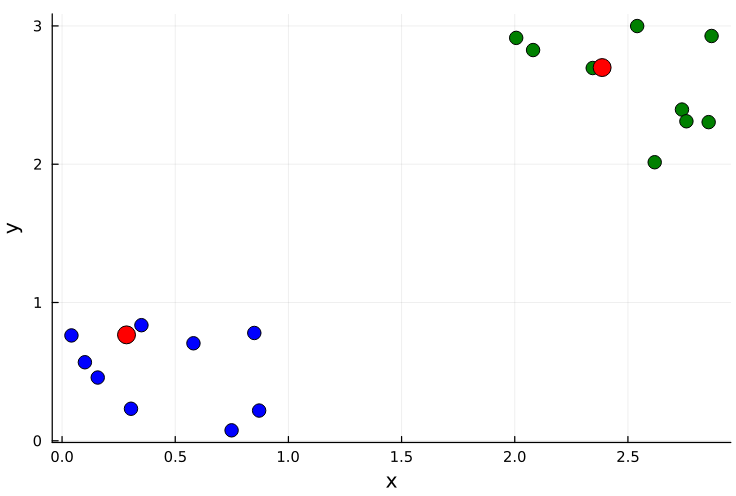
\includegraphics[width=8cm]{images/kmedoids2.png}
	\end{center}
\end{frame}

\begin{frame}[fragile]{Clustering Multivariate Data}{Problem of Distance Matrices}
\begin{lstlisting}
using Clustering, Plots, Distances

# data = Code for loading data...
plt = scatter(data[:, 1], data[:, 2])

dist = pairwise(euclidean, eachrow(data))

result = kmedoids(dist, 2)
centers = data[result.medoids, :];
scatter!(centers[:, 1], centers[:, 2])
\end{lstlisting}
\end{frame}

\subsection{Problem of Big Distance Matrices}

\begin{frame}[fragile]{A Distance Matrix}
$$
D = \begin{bmatrix}
D_{11} & D_{12} & D_{13} & \ldots & D_{1n} \\
D_{21} & D_{22} & D_{23} & \ldots & D_{2n} \\
\vdots & \vdots & \vdots & \ddots & \vdots \\
D_{n1} & D_{n2} & D_{n3} & \ldots & D_{nn} \\
\end{bmatrix}_{n \times n}
$$
\end{frame}

\begin{frame}[fragile]{Clustering Multivariate Data}{Problem of Distance Matrices}
\begin{lstlisting}
dist = pairwise(euclidean, eachrow(data))
\end{lstlisting}
\begin{itemize}
	\item A distance matrix holds the distance data of $ith$ and $jth$ points, e.g., $D_{ij} = D_{ji}$ due to the symmetry.
	\item If data has $n$ rows then the distance matrix is in dimension of $n \times n$. 
	\item Each distance is measured in 64-bits float numbers (\texttt{Float64}).
	\item If $n$ is large, your machine will probably throw an \emph{Out of Memory} error!
\end{itemize}
\end{frame}



\subsection{On-demand Distance Matrix}
\begin{frame}[fragile]{Big Distance Matrices}{On-demand Distance Matrix}
\begin{lstlisting}[basicstyle=\tiny]
struct OnDemandDistanceMatrix <: AbstractMatrix{Float64}
	rawdata::Matrix
end

function Base.getindex(odm::OnDemandDistanceMatrix, i::Int, j::Int)::Float64
	return euclidean(odm.rawdata[i, :], odm.rawdata[j, :])
end 

function Base.size(odm::OnDemandDistanceMatrix)
	n, _ = size(odm.rawdata)
	return (n, n)
end 
\end{lstlisting}
\end{frame} 


\begin{frame}[fragile]{Big Distance Matrices}{On-demand Distance Matrix}
\begin{lstlisting}
# Example 
data = Float64[
			1 2; 
			0 5; 
			1 2]

d = OnDemandDistanceMatrix(data)

println(d[1, 3])	
\end{lstlisting}
\end{frame} 


\begin{frame}[fragile]{Big Distance Matrices}{On-demand Distance Matrix}
\begin{lstlisting}
data = Float64[
		1 2; 
		0 5; 
		1 2]
		
d = OnDemandDistanceMatrix(data)
		
# d is a usual distance matrix now!
kmedoids(d, 2)	
\end{lstlisting}
\end{frame} 


\begin{frame}[fragile]{Big Distance Matrices}{On-demand Distance Matrix}
\begin{itemize}
	\item On-demand distance matrix costs zero memory
	\item Caution: But it's really slow just because the requested distance is calculated on demand!
	\item But it makes it possible! \Winkey
\end{itemize}
\end{frame} 

\subsection{Memory-mapped IO for Big Matrices}
\begin{frame}[fragile]{Big Matrices}{Memory Mapped IO}
	\begin{itemize}
		\item We need an efficient way to cope with big distance matrices 
		\item Memory-mapped IO is an OS level solution to this problem
		\item The content of a matrix is stored in files (on disk!)
		\item Access to data is really fast \Cooley (contrast to the previous one!)
	\end{itemize}
\end{frame} 

\begin{frame}[fragile]{Big Matrices}{Memory-mapped IO}
\begin{lstlisting}
import Mmap

xio = open("/tmp/X.dat", "w+")
yio = open("/tmp/y.dat", "w+")

X = Mmap.mmap(xio, Matrix{Float64}, (n, 2))
y = Mmap.mmap(yio, Vector{Float64}, n)		
\end{lstlisting}
\begin{itemize}
	\item $X$ and $y$ are stored in files \texttt{X.dat} and \texttt{y.dat}
	\item But they are stored in files and mapped to memory (RAM).
\end{itemize}
\end{frame}


\begin{frame}[fragile]{Big Matrices}{Memory-mapped IO}
$X$ and $y$ are processed and accessed as normal matrices and vectors
\begin{lstlisting}
X[1, :] = [1, 3]
y[5] = 9.7
betahats = inv(X'X)X'y
\end{lstlisting}
\end{frame}

\section{Distributions and Plots}
\begin{frame}[fragile]{Distributions}{The Normal Distribution}
\begin{equation}
f(x; \mu, \sigma) = \frac{1}{\sigma \sqrt{2\pi}} e^{-\frac{1}{2}\big(\frac{x - \mu}{\sigma}\big)^2}, \; -\infty < x < \infty
\end{equation}

\begin{equation}
	f(x; 0, 1) = \frac{1}{\sqrt{2\pi}} e^{-\frac{1}{2}x^2}, \; -\infty < x < \infty
\end{equation}
\end{frame}

\begin{frame}[fragile]{Distributions}{The Normal Distribution}
\begin{lstlisting}
julia> using Distributions

julia> quantile(Normal(), 0.05/2)
-1.9599639845400592

julia> quantile(Normal(), 0.10/2)
-1.6448536269514729

julia> quantile(Normal(), 0.01/2)
-2.5758293035489053
\end{lstlisting}
\end{frame}

\subsection{Monte Carlo Simulations}
\begin{frame}[fragile]{Distributions}{Monte Carlo Simulations - Drawing Random Numbers}
\begin{lstlisting}
julia> using Plots, Distributions
julia> x = rand(Normal(), 1000000);
julia> histogram(x)
\end{lstlisting}
\begin{center}
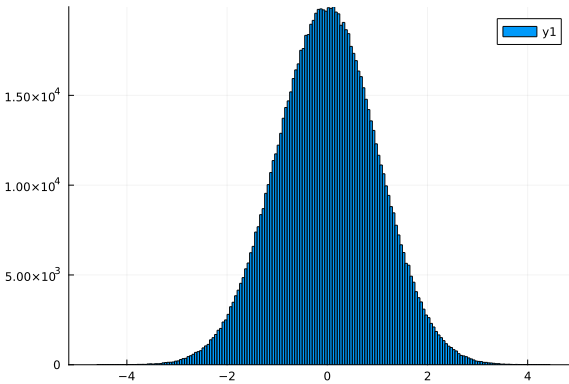
\includegraphics[width=7cm]{images/histogram.png}
\end{center}
\end{frame}

\begin{frame}[fragile]{Distributions}{Monte Carlo Simulations - Drawing Random Numbers}
	\begin{lstlisting}
julia> histogram(abs.(x))
	\end{lstlisting}
	\begin{center}
		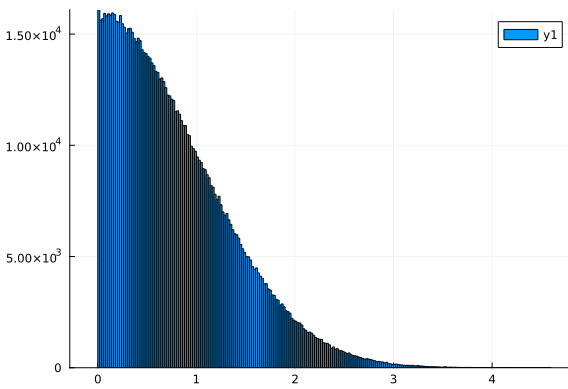
\includegraphics[width=7cm]{images/hist-abs-x.png}
	\end{center}
\end{frame}



\begin{frame}[fragile]{Hypothesis Tests}{Jarque-Bera Test for Normality}
\begin{lstlisting}
julia> using HypothesisTests
julia> x = randn(30);
julia> JarqueBeraTest(x)
\end{lstlisting}

The null hypothesis is a joint hypothesis of the skewness being $0$ and the kurtosis being $3$. 

$$
H_0: \text{Data comes from a Normal distribution}
$$

$$
H_a: \text{\Cat}
$$

\end{frame}

\begin{frame}[fragile]{Hypothesis Tests}{Jarque-Bera Test for Normality}
\begin{lstlisting}[basicstyle=\small]
Jarque-Bera normality test
--------------------------
Population details:
    parameter of interest:   skewness and kurtosis
    value under h_0:         "0 and 3"
    point estimate:          "-0.065 and 1.873"
Test summary:
    outcome with 95% confidence: fail to reject h_0
    one-sided p-value:           0.4474
Details:
    number of observations:         30
    JB statistic:                   1.60881
\end{lstlisting}
\end{frame}


\section{Numerical Integration}
\begin{frame}[fragile]{Numerical Integration}{QuadGK}
\begin{equation}
\int_{-1}^{1} \frac{1}{\sqrt{2\pi}} e^{-\frac{1}{2}x^2} dx = ?
\end{equation}
\begin{lstlisting}
using QuadGK

function f(x)
	return 1/sqrt(2pi) * exp(-0.5x^2)
end 

quadgk(f, -1.0, 1.0)
\end{lstlisting}
\end{frame}

\section{Optimizations}

\subsection{The Simple Neural Network}
\begin{frame}[fragile]{Optimizations}{Simple Neural Network}
\begin{center}
$$
H_1 = f(w_0 + x_1w_{11} + x_2w_{21})
$$
 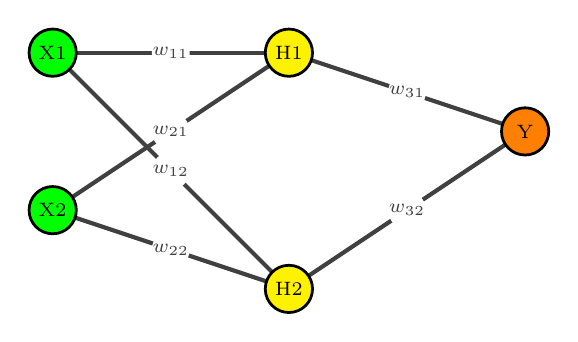
\begin{tikzpicture}
	\Vertex[x=0,y=0,color=green,label=X1]{X1} 
	\Vertex[x=0,y=-2,color=green,label=X2]{X2}
	\Vertex[x=3,y=0,color=yellow, label=H1]{H1}
	 \Vertex[x=3,y=-3,color=yellow, label=H2]{H2}
	\Vertex[x=6,y=-1,color=orange,label=Y]{Y} 
	
	\Edge[Math,label=w_{11}](X1)(H1)
	\Edge[Math,label=w_{12}](X1)(H2)
	\Edge[Math,label=w_{21}](X2)(H1)
	\Edge[Math,label=w_{22}](X2)(H2)
	\Edge[Math,label=w_{31}](H1)(Y)
	\Edge[Math,label=w_{32}](H2)(Y)
\end{tikzpicture}
\end{center}
\end{frame}

\begin{frame}[fragile]{Optimizations}{Simple Neural Network}

$$
H_1 = f(w_{01} + x_1w_{11} + x_2w_{21})
$$

$$
H_2 = f(w_{02} + x_1w_{12} + x_2w_{22})
$$

$$
Y = f(w_{03} + w_{31}H_1 + w_{32}H_2)
$$

What are the values of $w_{ij}$'s that minimize the total network error?
\end{frame}

\begin{frame}[fragile]{Optimizations}{Simple Neural Network}
\begin{lstlisting}[basicstyle=\tiny]
function sigmoid(x)
	return 1.0/(1.0 + exp(-x))
end 

function cost(w)
	error = 0.0
	for i in 1:4
		H1 = sigmoid(w[1] + w[2]*x1[i] + w[3]*x2[i])
		H2 = sigmoid(w[4] + w[5]*x1[i] + w[6]*x2[i])
		yhat = sigmoid(w[7] + w[8] * H1 + w[9] * H2)
		error += (yhat - y[i])^2
	end 
	return error 
end 
\end{lstlisting}
\end{frame}

\begin{frame}[fragile]{Optimizations}{Simple Neural Network}
\begin{lstlisting}[basicstyle=\small]
using Metaheuristics 

x1 = [1, 1, 0, 0]
x2 = [1, 0, 1, 0]
y  = [0, 1, 1, 0]

bounds = vcat([-10000.0 for i in 1:9]', 
			  [10000.0 for i in 1:9]')

result = Metaheuristics.optimize(cost, bounds, MCCGA())

display(result)
\end{lstlisting}
\end{frame}

\begin{frame}[fragile]{Feeding the trained network}
\begin{lstlisting}[basicstyle=\small]
function forward(w)
	yhat = zeros(length(y))
	for i in 1:4
		H1 = sigmoid(w[1] + w[2]*x1[i] + w[3]*x2[i])
		H2 = sigmoid(w[4] + w[5]*x1[i] + w[6]*x2[i])
		H3 = sigmoid(w[7] + w[8] * H1 + w[9] * H2)
		yhat[i] = H3
	end 
	return yhat
end 
\end{lstlisting}
\end{frame}

\subsection{Mathematical Programming}
\begin{frame}[fragile]{Optimizations}{Mathematical Programming}
$$
\begin{aligned}
\max z = & 2x_1 + 3x_2 \\
\text{Subject to:}\\
& x_1 + 2x_2 \le 100 \\
& 2x_1 + x_2 \le 150 \\
& x_1, x_2 \ge 0
\end{aligned}
$$
\end{frame}

\begin{frame}[fragile]{Optimizations}{JuMP}
\begin{lstlisting}[basicstyle=\small]
using JuMP, HiGHS

m = Model(HiGHS.Optimizer)

@variable(m, x1 >= 0)
@variable(m, x2 >= 0)

@objective(m, Max, 2x1 + 3x2)

@constraint(m, x1 + 2x2 <= 100)
@constraint(m, 2x1 + x2 <= 150)
\end{lstlisting}
\end{frame}


\begin{frame}[fragile]{Optimizations}{JuMP}
\begin{lstlisting}
julia> optimize!(m)
Solving LP without presolve or with basis
Model   status      : Optimal
Objective value     :  1.8333333333e+02
HiGHS run time      :          0.00

julia> value.([x1, x2])
2-element Vector{Float64}:
66.66666666666667
16.666666666666657	
\end{lstlisting}
\end{frame}

\section{SQL}
\begin{frame}[fragile]{SQL Integration}{SQLite}
\begin{lstlisting}[basicstyle=\tiny]
using SQLite

db = SQLite.DB("database.db")

sqlst = """ 
	select item, price from Prices 
	where date = '2023.12.01' 
	order by price
"""

resultsql = DBInterface.execute(db, sqlst)

for row in resultsql
	println(row[:item], ": ", row[:price])
end 

close(db)
\end{lstlisting}
\end{frame}


\section{Talking to Strangers}

\begin{frame} 
\begin{itemize}
\item Julia can operate with R and Python.
\item R and Python objects can be transferred in both ways.
\item We don't need to give up on them, let's talk to the strangers!
\end{itemize}
\end{frame}

\subsection{Calling R from within Julia}
\begin{frame}[fragile]{Talking to Strangers}{Calling into R}
\begin{lstlisting}
using RCall

x = [1, 2, 3, 4, 5]
y = [2, 5, 5, 8, 12]

@rput x y

R"result <- lm(y~x)"

jresult = @rget result
\end{lstlisting}
\end{frame}

\begin{frame}[fragile]
\begin{lstlisting}
julia> jresult
  :coefficients  => [-0.5, 2.3]
  :residuals     => [0.2, 0.9, -1.4, -0.7, 1.0]
  :rank          => 2
  :fitted_values => [1.8, 4.1, 6.4, 8.7, 11.0]
  :assign        => [0, 1]
  :df_residual   => 3
  :xlevels       => OrderedDict{Symbol, Any}()
  :terms         => y ~ x
\end{lstlisting}
\end{frame}


\subsection{Calling Python from within Julia}
\begin{frame}[fragile]{Talking to Strangers}{Calling into Python}
\begin{lstlisting}
using PyCall

np = pyimport("numpy")
linalg = pyimport("numpy.linalg")

x = np.matrix([1.0 1; 1 2; 1 3; 1 4; 1 5])
y = np.array([2.0, 5, 5, 8, 12])

result = linalg.lstsq(x, y)
\end{lstlisting}
\end{frame}

\begin{frame}[fragile]{Talking to Strangers}{Calling into Python}
\begin{lstlisting}
julia> include("pycaller.jl")
(
	[-0.5000000000000023, 2.3000000000000003], 
	[4.299999999999995], 
	 2, 
	[7.69121313410482, 0.9193696350073228]
)
\end{lstlisting}
\end{frame}



\section{Conclusion and Questions}
\begin{frame}
\begin{center}

\includegraphics[width=1cm]{images/julia.png}

Thank you!

Any questions? \Coffeecup
\end{center}
\end{frame}

\end{document}